\section{Data model}
\label{sec:model}

\paragraph{Atoms.} Everything HStore stores is an \emph{atom} with a 64-bit identifier, handed out in increasing order. An atom is a \emph{node} or a \emph{hyperedge}. Both have a type, both can have properties, and a node can also have a canonical key that is unique within its type, such as \code{Person:'alice'}.

\paragraph{Hyperedges and incidences.} A hyperedge has any number of members. Each membership is an \emph{incidence}
\[
(\mathit{member}, \mathit{roles}, \mathit{weight}, [\mathit{from}, \mathit{to}), \mathit{data}, \mathit{qualifier}),
\]
where $\mathit{member}$ is any atom, including another hyperedge; $\mathit{roles}$ is a set of role names (a member can be both buyer and approver); $\mathit{weight}$ is an exact fixed-point number with nine decimal places; $[\mathit{from}, \mathit{to})$ is the interval in which the membership holds; $\mathit{data}$ points to a payload and $\mathit{qualifier}$ to an atom that records evidence for it. All fields except the member have defaults. A \emph{set} hyperedge holds each atom at most once and has no order. An \emph{ordered} hyperedge is a sequence that can be edited at any position, and the same atom can appear in it only once.

\begin{figure*}[t]
\centering
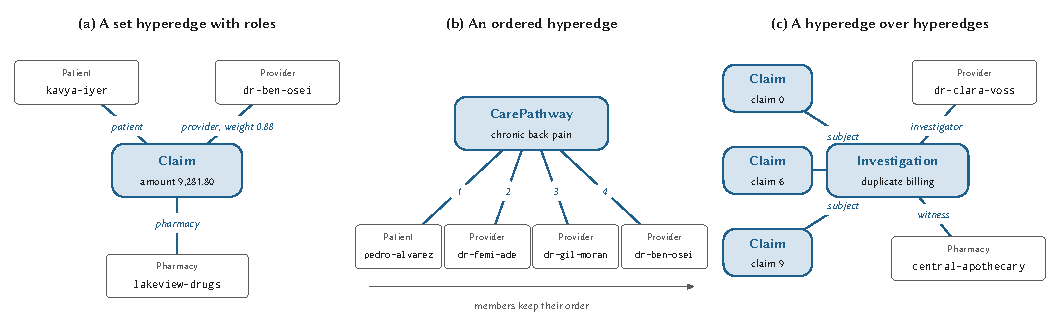
\includegraphics[width=\textwidth]{figures/hypergraph}
\caption{Three hyperedges from the clinical claims example that ships with HStore. (a) A claim relates a patient, a provider and a pharmacy, each in its own role; the provider's membership carries a weight. (b) A care pathway lists a patient and the providers who saw them, in order. (c) An investigation has three claims as its subjects, so its members are themselves hyperedges.}
\label{fig:hypergraph}
\end{figure*}

\Cref{fig:hypergraph} shows one hyperedge of each kind from the example dataset that ships with HStore.

\paragraph{Generations, history and branches.} Every commit produces a new \emph{generation}, numbered consecutively. A reader opens a snapshot of a generation and sees it unchanged for as long as it keeps it open. The engine keeps a configurable number of recent generations (64 by default) for time travel, which can be addressed by number or by wall-clock time. A \emph{branch} is a named line of generations forked from another branch. Creating one copies nothing, and the database layer merges branches with a three-way merge against the fork point.

\paragraph{Operations.} Writes create and delete atoms, change their records, and change memberships: add, update or remove a member by atom, insert, update or remove at a position in an ordered hyperedge, and replace a whole membership in one bulk load. Deleting an atom removes it from every hyperedge that contains it. Reads look up an atom, test and fetch a member, return a hyperedge's cardinality and the member at a given rank, scan members filtered by role, weight or validity time, list the hyperedges incident to an atom, intersect incidence sets (``hyperedges that contain all of $a_1,\dots,a_k$''), and compute differences between two hyperedges, two generations or two branches.

\paragraph{Layers.} The storage engine knows only atoms, memberships and a set of keyed trees. Types, property values, tenants and users, the HQL query language, an embedding index and the higher-order operators are added by a database layer that stores its own data in additional trees inside the same generations (\cref{sec:implementation}). The rest of this paper is about the engine.
